\chapter{Märkte und Marktinterventionen}

\section{Märkte}

\begin{definition}
	Gegeben seien eine Nachfragefunktion $D(p)$ und eine Angebotsfunktion $S(p)$ für ein Gut auf einem isolierten Markt.
	Ein partielles Marktgleichgewicht ist ein Preis-Mengen-Paar $(p^*,q^*)$, so dass gilt:
	\[
		D(p^*) = S(p^*) = q^*
		.\]
\end{definition}

Betrachten wir die Stabilitätsbedingung, das heißt, wenn gilt
\[
	\frac{\mathrm{d}}{\mathrm{d}p} \left( S(p) -D(p) \right) \mid_{p=p^*} > 0
	.\]
Dies führt dazu, dass ein Preisanstieg oberhalb $p^*$ zu einem Angebotsüberschuss führt.
Analog geht mit einem Preisrückgang ein Nachfrageüberschuss einher.


\begin{figure}[h]
	\caption{partielles Marktgleichgewicht, mit linearen Nachfrage- und Angebotskurve}
	\begin{center}
		\begin{tikzpicture}[scale=1.2]
			% Achsen
			\draw[->] (0,0) -- (6,0) node[right] {Menge $q$};
			\draw[->] (0,0) -- (0,5) node[above] {Preis $p$};

			% Nachfragefunktion D(p)
			\draw[thick,blue] (0.5,4.5) -- (5.5,0.5) node[below right] {$D(p)$};

			% Angebotsfunktion S(p)
			\draw[thick,red] (0.5,0.5) -- (5.5,4.5) node[above right] {$S(p)$};

			% Gleichgewichtspunkt
			\draw[dashed] (3,0) -- (3,2.5);
			\draw[dashed] (0,2.5) -- (3,2.5);
			\filldraw[black] (3,2.5) circle (2pt) node[above right] {$(q^*, p^*)$};

			% Achsenbeschriftungen
			\node at (3,-0.3) {$q^*$};
			\node at (-0.3,2.5) {$p^*$};

		\end{tikzpicture}

	\end{center}
\end{figure}

Das partielle Marktgleichgewicht kann benutzt werden um zu analysieren was passiert, wenn sich Angebot oder Nachfrage verändern.
Eine solche Analyse als komperative Statik bezeichnet.

\begin{figure}
	\begin{center}
		\caption{Nachfrage und Angebotsveränderung}
		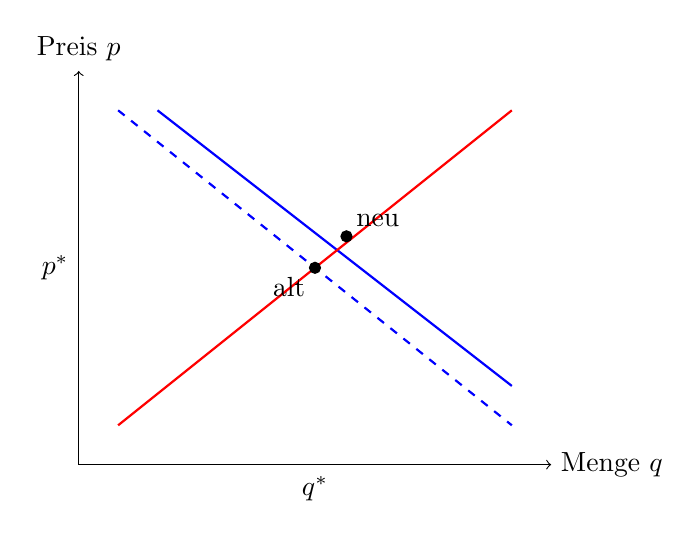
\begin{tikzpicture}[scale=1]
			% Achsen
			\draw[->] (0,0) -- (6,0) node[right] {Menge $q$};
			\draw[->] (0,0) -- (0,5) node[above] {Preis $p$};

			% Alte Nachfrage
			\draw[thick,blue,dashed] (0.5,4.5) -- (5.5,0.5);

			% Neue Nachfrage
			\draw[thick,blue] (1,4.5) -- (5.5,1);

			% Angebot
			\draw[thick,red] (0.5,0.5) -- (5.5,4.5);

			% Gleichgewichtspunkte
			\filldraw[black] (3,2.5) circle (2pt) node[below left] {alt};
			\filldraw[black] (3.4,2.9) circle (2pt) node[above right] {neu};

			% Achsenbeschriftungen
			\node at (3,-0.3) {$q^*$};
			\node at (-0.3,2.5) {$p^*$};

		\end{tikzpicture}



		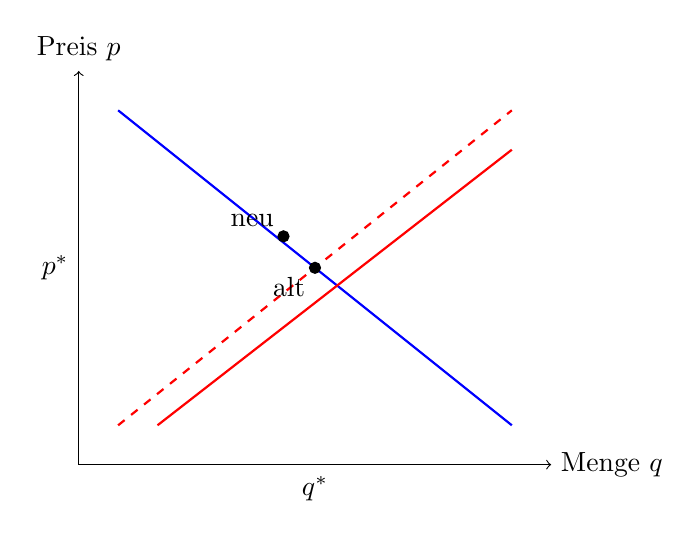
\begin{tikzpicture}[scale=1]
			% Achsen
			\draw[->] (0,0) -- (6,0) node[right] {Menge $q$};
			\draw[->] (0,0) -- (0,5) node[above] {Preis $p$};

			% Nachfrage
			\draw[thick,blue] (0.5,4.5) -- (5.5,0.5);

			% Altes Angebot
			\draw[thick,red,dashed] (0.5,0.5) -- (5.5,4.5);

			% Neues Angebot (linksverschoben)
			\draw[thick,red] (1,0.5) -- (5.5,4);

			% Gleichgewichtspunkte
			\filldraw[black] (3,2.5) circle (2pt) node[below left] {alt};
			\filldraw[black] (2.6,2.9) circle (2pt) node[above left] {neu};

			% Achsenbeschriftungen
			\node at (3,-0.3) {$q^*$};
			\node at (-0.3,2.5) {$p^*$};

		\end{tikzpicture}

	\end{center}

\end{figure}


\section{Marktinterventionen}



In unserem bisherigem vorgehen, haben wir staatliche Eingriffe oder andere Friktionen vernachlässigt.
Typischerweise existieren diese, oft sind diese Eingriffe Steuern.

\subsection{Steuern}

%Mengensteuer


\subsection{Zölle und Quoten}

Damit wir Zöllen und Quoten überhaupt behandeln können, müssen wir handel zu lassen.


\begin{definition} \index{Freihandel}
	Eine Situation, in der uneingeschränkt gehandelt werden kann, wird als
	\defemph{Freihandel} bezeichnet.
\end{definition}

Handel ergibt nur Sinn, wenn der internationale Angebotspreis unterhalb des lokalen Angebotspreis ist.


Neben Zoll auf die Güter, kann es auch Quoten geben, die den Import auf gewisse Güter auf eine Menge beschränkt wird.
